\documentclass{standalone}
\usepackage{tikz}
\usetikzlibrary{patterns, positioning}
\usepackage[sfdefault]{ClearSans} %% option 'sfdefault' activates Clear Sans as the default text font
\usepackage[T1]{fontenc}

\begin{document}
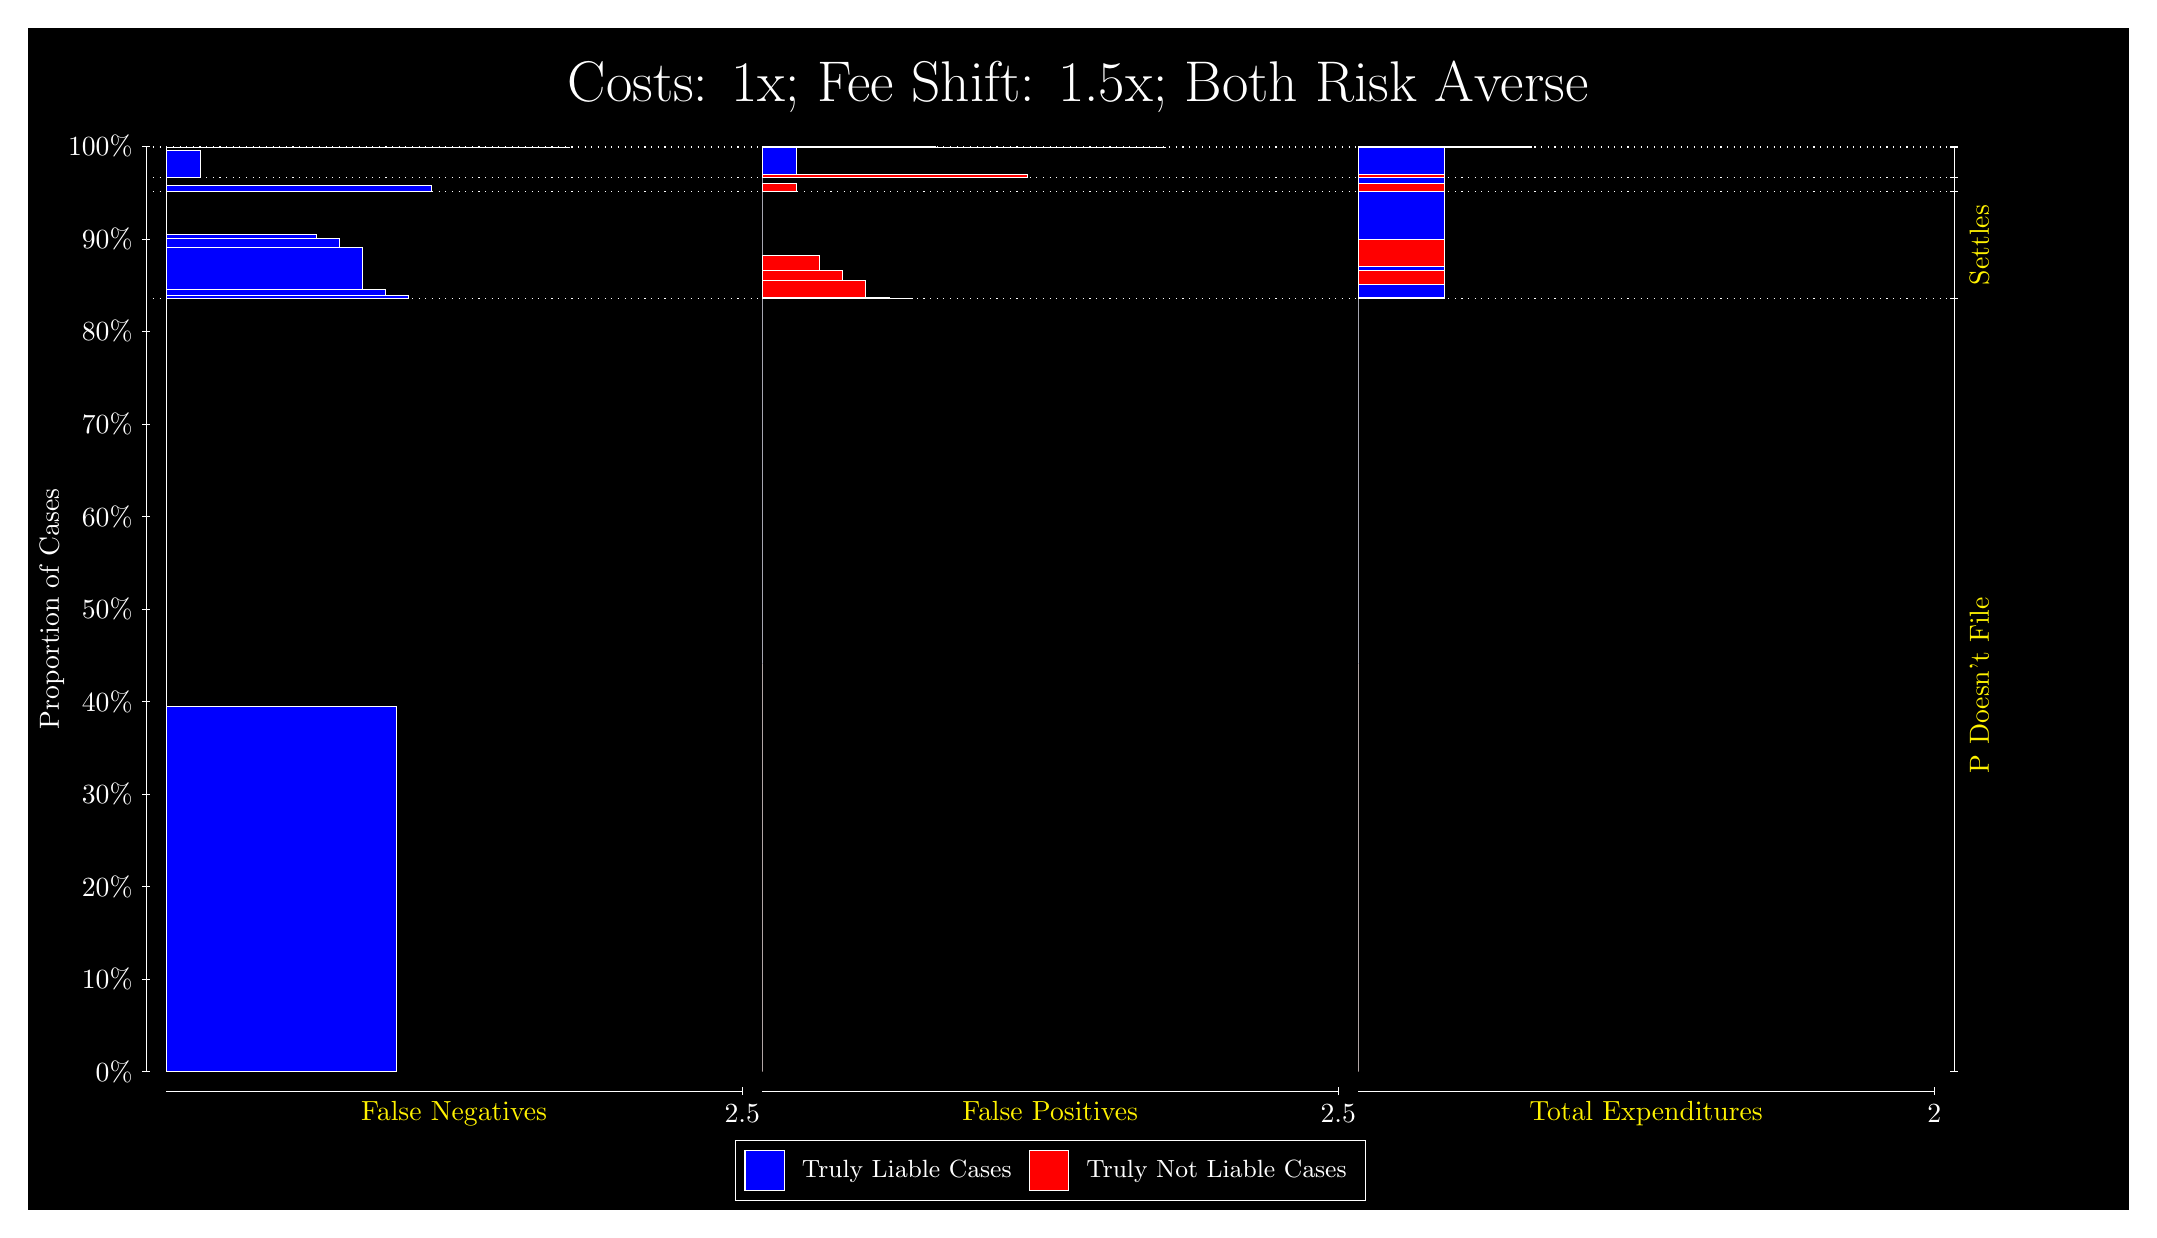
\begin{tikzpicture}
\draw[fill=black] (0,0) rectangle (26.667,15);
\draw[text=white] (0,13.5) rectangle (26.667,15) node[midway] {\huge Costs: 1x; Fee Shift: 1.5x; Both Risk Averse};
\draw[white, very thin] (1.5,1.75) -- (1.5,13.5);
\node[rotate=90, text=white, anchor=center] at (0.3, 7.625) {Proportion of Cases};
\draw[white, very thin] (1.45,1.75) -- (1.55,1.75);
\node[text=white, anchor=east] at (1.45, 1.75) {0\%};
\draw[white, very thin] (1.45,2.925) -- (1.55,2.925);
\node[text=white, anchor=east] at (1.45, 2.925) {10\%};
\draw[white, very thin] (1.45,4.1) -- (1.55,4.1);
\node[text=white, anchor=east] at (1.45, 4.1) {20\%};
\draw[white, very thin] (1.45,5.275) -- (1.55,5.275);
\node[text=white, anchor=east] at (1.45, 5.275) {30\%};
\draw[white, very thin] (1.45,6.45) -- (1.55,6.45);
\node[text=white, anchor=east] at (1.45, 6.45) {40\%};
\draw[white, very thin] (1.45,7.625) -- (1.55,7.625);
\node[text=white, anchor=east] at (1.45, 7.625) {50\%};
\draw[white, very thin] (1.45,8.8) -- (1.55,8.8);
\node[text=white, anchor=east] at (1.45, 8.8) {60\%};
\draw[white, very thin] (1.45,9.975) -- (1.55,9.975);
\node[text=white, anchor=east] at (1.45, 9.975) {70\%};
\draw[white, very thin] (1.45,11.15) -- (1.55,11.15);
\node[text=white, anchor=east] at (1.45, 11.15) {80\%};
\draw[white, very thin] (1.45,12.325) -- (1.55,12.325);
\node[text=white, anchor=east] at (1.45, 12.325) {90\%};
\draw[white, very thin] (1.45,13.5) -- (1.55,13.5);
\node[text=white, anchor=east] at (1.45, 13.5) {100\%};

\draw[white, very thin] (24.457,1.75) -- (24.457,13.5);
\draw[white, very thin] (24.407,1.75) -- (24.507,1.75);
\node[anchor=west] at (24.407, 1.75) {};
\draw[white, very thin] (24.407,11.565) -- (24.507,11.565);
\node[anchor=west] at (24.407, 11.565) {};
\draw[white, very thin] (24.407,12.926) -- (24.507,12.926);
\node[anchor=west] at (24.407, 12.926) {};
\draw[white, very thin] (24.407,13.107) -- (24.507,13.107);
\node[anchor=west] at (24.407, 13.107) {};
\draw[white, very thin] (24.407,13.487) -- (24.507,13.487);
\node[anchor=west] at (24.407, 13.487) {};
\draw[white, very thin] (24.407,13.491) -- (24.507,13.491);
\node[anchor=west] at (24.407, 13.491) {};
\draw[white, very thin] (24.407,13.5) -- (24.507,13.5);
\node[anchor=west] at (24.407, 13.5) {};

\draw[white, very thin, fill=blue] (1.75,1.75) rectangle (4.6775,6.385);
\draw[white, very thin, fill=red] (1.75,6.385) rectangle (1.75,11.565);
\draw[white, very thin, fill=blue] (1.75,11.565) rectangle (4.8239,11.609);
\draw[white, very thin, fill=blue] (1.75,11.609) rectangle (4.5312,11.687);
\draw[white, very thin, fill=blue] (1.75,11.687) rectangle (4.2384,12.216);
\draw[white, very thin, fill=blue] (1.75,12.216) rectangle (3.9457,12.327);
\draw[white, very thin, fill=blue] (1.75,12.327) rectangle (3.6529,12.38);
\draw[white, very thin, fill=red] (1.75,12.38) rectangle (1.75,12.926);
\draw[white, very thin, fill=blue] (1.75,12.926) rectangle (5.1167,13);
\draw[white, very thin, fill=red] (1.75,13) rectangle (1.75,13.107);
\draw[white, very thin, fill=blue] (1.75,13.107) rectangle (2.1891,13.45);
\draw[white, very thin, fill=red] (1.75,13.45) rectangle (1.75,13.487);
\draw[white, very thin, fill=blue] (1.75,13.487) rectangle (6.8732,13.489);
\draw[white, very thin, fill=red] (1.75,13.489) rectangle (1.75,13.491);
\draw[white, very thin, fill=red] (1.75,13.491) rectangle (1.75,13.493);
\draw[white, very thin, fill=blue] (1.75,13.493) rectangle (1.75,13.5);
\draw[white, very thin, fill=red] (9.3189,1.75) rectangle (9.3189,6.9297);
\draw[white, very thin, fill=blue] (9.3189,6.9297) rectangle (9.3189,11.565);
\draw[white, very thin, fill=red] (9.3189,11.565) rectangle (11.222,11.569);
\draw[white, very thin, fill=red] (9.3189,11.569) rectangle (10.929,11.584);
\draw[white, very thin, fill=red] (9.3189,11.584) rectangle (10.636,11.798);
\draw[white, very thin, fill=red] (9.3189,11.798) rectangle (10.344,11.931);
\draw[white, very thin, fill=red] (9.3189,11.931) rectangle (10.051,12.111);
\draw[white, very thin, fill=blue] (9.3189,12.111) rectangle (9.3189,12.926);
\draw[white, very thin, fill=red] (9.3189,12.926) rectangle (9.758,13.033);
\draw[white, very thin, fill=blue] (9.3189,13.033) rectangle (9.3189,13.107);
\draw[white, very thin, fill=red] (9.3189,13.107) rectangle (12.686,13.145);
\draw[white, very thin, fill=blue] (9.3189,13.145) rectangle (9.758,13.487);
\draw[white, very thin, fill=red] (9.3189,13.487) rectangle (9.3189,13.489);
\draw[white, very thin, fill=blue] (9.3189,13.489) rectangle (9.3189,13.491);
\draw[white, very thin, fill=red] (9.3189,13.491) rectangle (14.442,13.493);
\draw[white, very thin, fill=blue] (9.3189,13.493) rectangle (11.515,13.5);
\draw[white, very thin, fill=red] (16.888,1.75) rectangle (16.888,6.9297);
\draw[white, very thin, fill=blue] (16.888,6.9297) rectangle (16.888,11.565);
\draw[white, very thin, fill=red] (16.888,11.565) rectangle (17.986,11.584);
\draw[white, very thin, fill=blue] (16.888,11.584) rectangle (17.986,11.747);
\draw[white, very thin, fill=red] (16.888,11.747) rectangle (17.986,11.928);
\draw[white, very thin, fill=blue] (16.888,11.928) rectangle (17.986,11.972);
\draw[white, very thin, fill=red] (16.888,11.972) rectangle (17.986,12.319);
\draw[white, very thin, fill=blue] (16.888,12.319) rectangle (17.986,12.926);
\draw[white, very thin, fill=red] (16.888,12.926) rectangle (17.986,13.033);
\draw[white, very thin, fill=blue] (16.888,13.033) rectangle (17.986,13.107);
\draw[white, very thin, fill=red] (16.888,13.107) rectangle (17.986,13.145);
\draw[white, very thin, fill=blue] (16.888,13.145) rectangle (17.986,13.487);
\draw[white, very thin, fill=red] (16.888,13.487) rectangle (19.083,13.489);
\draw[white, very thin, fill=blue] (16.888,13.489) rectangle (19.083,13.491);
\draw[white, very thin, fill=red] (16.888,13.491) rectangle (19.083,13.493);
\draw[white, very thin, fill=blue] (16.888,13.493) rectangle (19.083,13.5);
\draw[white, dotted] (1.5,11.565) -- (24.457,11.565);
\draw[white, dotted] (1.5,12.926) -- (24.457,12.926);
\draw[white, dotted] (1.5,13.107) -- (24.457,13.107);
\draw[white, dotted] (1.5,13.487) -- (24.457,13.487);
\draw[white, dotted] (1.5,13.491) -- (24.457,13.491);
\draw[white, very thin] (1.75,1.5) -- (9.0689,1.5);
\node[text=yellow, anchor=north] at (5.4094, 1.5) {False Negatives};
\draw[white, very thin] (9.0689,1.45) -- (9.0689,1.55);
\node[text=white, anchor=north] at (9.0689, 1.45) {2.5};

\draw[white, very thin] (9.3189,1.5) -- (16.638,1.5);
\node[text=yellow, anchor=north] at (12.978, 1.5) {False Positives};
\draw[white, very thin] (16.638,1.45) -- (16.638,1.55);
\node[text=white, anchor=north] at (16.638, 1.45) {2.5};

\draw[white, very thin] (16.888,1.5) -- (24.207,1.5);
\node[text=yellow, anchor=north] at (20.547, 1.5) {Total Expenditures};
\draw[white, very thin] (24.207,1.45) -- (24.207,1.55);
\node[text=white, anchor=north] at (24.207, 1.45) {2};

\node[text=yellow, centered, rotate=90] at (24.777, 6.6573) {P Doesn't File};
\node[text=yellow, centered, rotate=90] at (24.777, 12.246) {Settles};





\draw (12.978300999999998,1.5) node[draw=none] (baseCoordinate) {};
\begin{scope}[align=center]
        \matrix[scale=0.5, draw=white, below=0.5cm of baseCoordinate, nodes={draw}, column sep=0.1cm]{
            \node[rectangle, draw, minimum width=0.5cm, minimum height=0.5cm, fill=blue] {}; &
            \node[draw=none, font=\small, text=white] (B) {Truly Liable Cases}; &
            \node[rectangle, draw, minimum width=0.5cm, minimum height=0.5cm, fill=red] {}; &
            \node[draw=none, font=\small, text=white] (B) {Truly Not Liable Cases}; \\
            };
\end{scope}

\end{tikzpicture}
\end{document}